The scenario damage calculator computes damage distribution statistics for all
assets in a given \gls{exposuremodel} for a single specified earthquake
rupture. Damage distribution statistics include the mean and standard
deviation of damage fractions for different damage states. This calculator
requires the definition of a finite rupture model, an \gls{exposuremodel} and
a \gls{fragilitymodel}; the main results are the damage distribution
statistics per asset, aggregated damage distribution statistics per taxonomy,
aggregated damage distribution statistics for the region, and collapse maps,
which contain the spatial distribution of the number or area of collapsed
buildings throughout the region of interest.

The rupture characteristics---i.e. the magnitude, hypocenter and fault
geometry---are modelled as deterministic in the scenario calculators. Multiple
realizations of different possible ground motion fields (GMFs) due to the
single rupture are generated, taking into consideration both the inter-event
variability of ground motions, and the intra-event residuals obtained from a
spatial correlation model for ground motion residuals. The use of logic trees
allows for the consideration of uncertainty in the choice of a ground motion
model for the given tectonic region.

As an alternative to computing the GMFs with \glsdesc{acr:oqe}, users can also
provide their own sets of GMFs as input to the scenario damage calculator.

For each GMF realization, damage fractions (the fraction of buildings in each
damage state) are estimated for every asset in the \gls{exposuremodel} using the
provided fragility model, and finally the damage distribution statistics
(i.e., the mean damage fractions and standard deviation of damage fractions
for all damage states) across all realizations are calculated. The calculator
also provides aggregated damage distribution statistics for the portfolio,
such as mean damage fractions and standard deviation of damage fractions for
each taxonomy in the \gls{exposuremodel}, and the mean damage fractions and
standard deviation of damage fractions for the entire region of study.

The required input files required for running a scenario damage calculation
and the resulting output files are depicted in Figure~\ref{fig:io-structure-scenario-damage}.

\begin{figure}[ht]
\centering
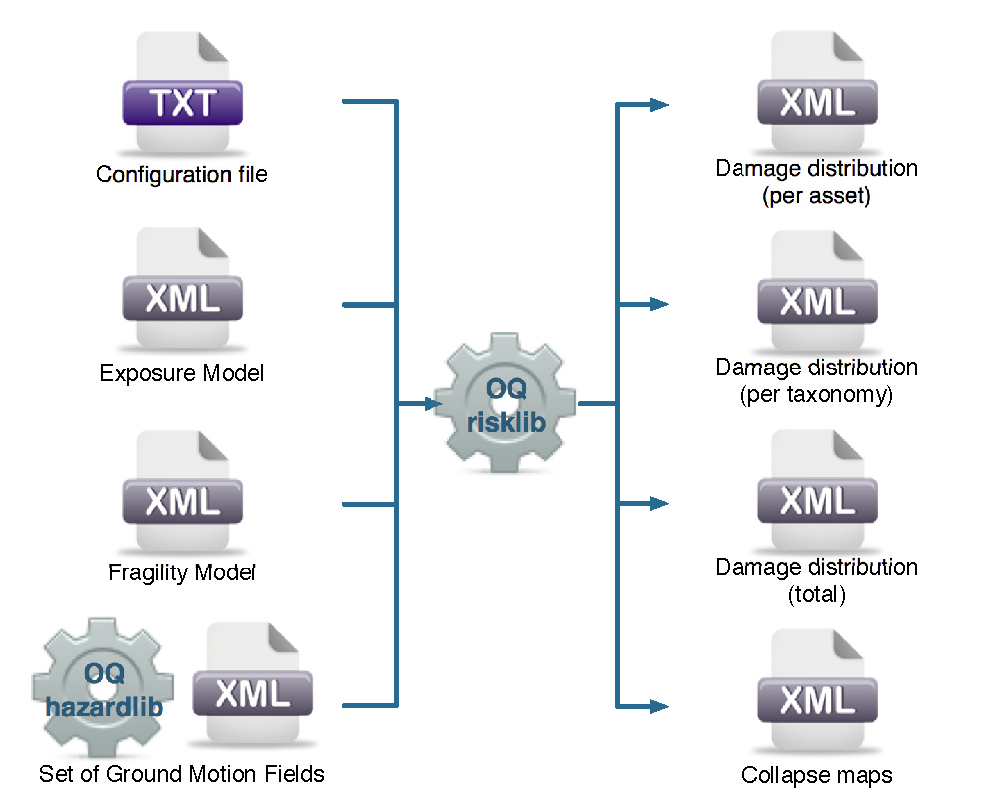
\includegraphics[width=9cm,height=7cm]{figures/risk/io-structure-scenario-damage.pdf}
\caption{Scenario Damage Calculator input/output structure.}
\label{fig:io-structure-scenario-damage}
\end{figure}

Starting with \glsdesc{acr:oqe17}, \gls{consequencemodel} files can also be
provided as inputs for a scenario damage calculation in addition to
\glspl{fragilitymodel} files, in order to estimate consequences based on the
calculated damage distribution. The user may provide one
\gls{consequencemodel} file corresponding to each loss type (amongst structural,
nonstructural, contents, and business interruption) for which a fragility
model file is provided. Whereas providing a \gls{fragilitymodel} file for at
least one loss type is mandatory for running a Scenario Damage calculation,
providing corresponding \gls{consequencemodel} files is optional.
